\documentclass[9pt]{beamer}
\usepackage{url}
\usetheme[progressbar=frametitle]{metropolis}
\usepackage{appendixnumberbeamer}
\usepackage[numbers,sort&compress]{natbib}
\bibliographystyle{plainnat}
\usepackage{subfig}
\usepackage{booktabs}
\usepackage[scale=2]{ccicons}

\usepackage{xspace}
\newcommand{\themename}{\textbf{\textsc{metropolis}}\xspace}

\AtBeginSection[]
{
  \begin{frame}
    \frametitle{Table of Contents}
    \tableofcontents[currentsection]
  \end{frame}
}




\title{TURLA\\LIGHTNEURON}
\subtitle{One email away from remote code execution}
% \date{\today}
\date{}
\author{Mario Leonardo Salinas}
\institute{UniPi - ICT Risk Assessment}
% \titlegraphic{\hfill\includegraphics[height=1.5cm]{logo.pdf}}

\begin{document}

\maketitle

\begin{frame}{Table of contents}
  \setbeamertemplate{section in toc}[sections numbered]
  \tableofcontents[hideallsubsections]
\end{frame}
%============================
%   1. Introduction
%============================
\section{Introduction}

\begin{frame}[fragile]{Metropolis}
  The \themename theme is a Beamer theme \cite{greenwade93} with minimal visual noise
  inspired by the \href{https://github.com/hsrmbeamertheme/hsrmbeamertheme}{\textsc{hsrm} Beamer
  Theme} by Benjamin Weiss. \cite{Er01}

  Enable the theme \cite{Simpson} by loading

  \begin{verbatim}    \documentclass{beamer}
    \usetheme{metropolis}\end{verbatim}

  Note, that you have to have Mozilla's \emph{Fira Sans} font and XeTeX
  installed to enjoy this wonderful typography.
\end{frame}
%============================
%   2. Attacker Profile & Victimology
%============================
\section{Attacker Profile \& Victimology}

\begin{frame}[fragile]{Attacker Profile i}
  \begin{itemize}
    \item Turla is well known for its advanced custom tools and its ability to run highly targeted operations.
    \item The group is interested in collecting information from strategic people
    or organizations.
  \end{itemize}
  \begin{figure}
    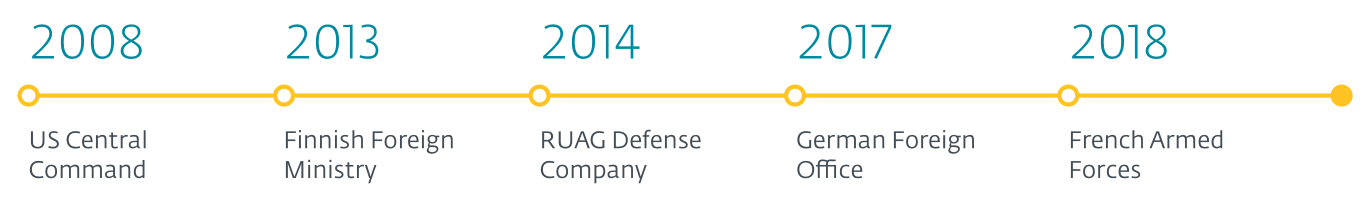
\includegraphics[width=\textwidth]{figures/timeline.PNG}
    \caption{Timeline of important attacks attributed to Turla}
  \end{figure}
\end{frame}

\begin{frame}[fragile]{Attacker Profile ii}
    \begin{itemize}
      \item The operators activity matches a typical 9-to-5 workday in the UTC+3 time zone
      \item LightNeuron is used mostly to exfiltrate data. The remaining activity is most likely dropping
      and executing tools to perform lateral movements across the local network
    \end{itemize}
    \begin{figure}
      \centering
      \subfloat[Operators working hours\label{fig:a}]{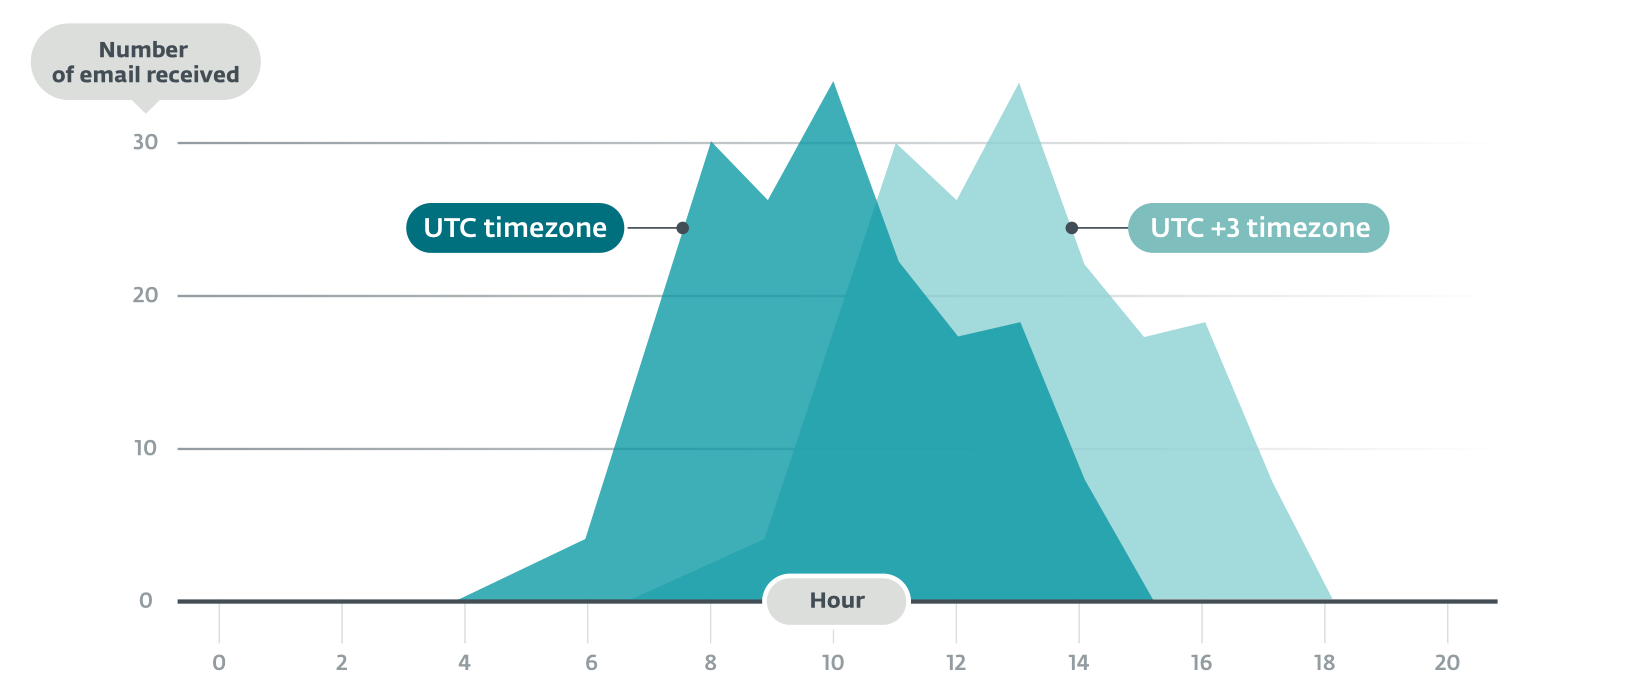
\includegraphics[height=3.5cm,width=5.5cm]{figures/attacker_timeline.PNG}}\qquad
      \subfloat[Distribution of the backdoor commands used by the operators\label{fig:b}]{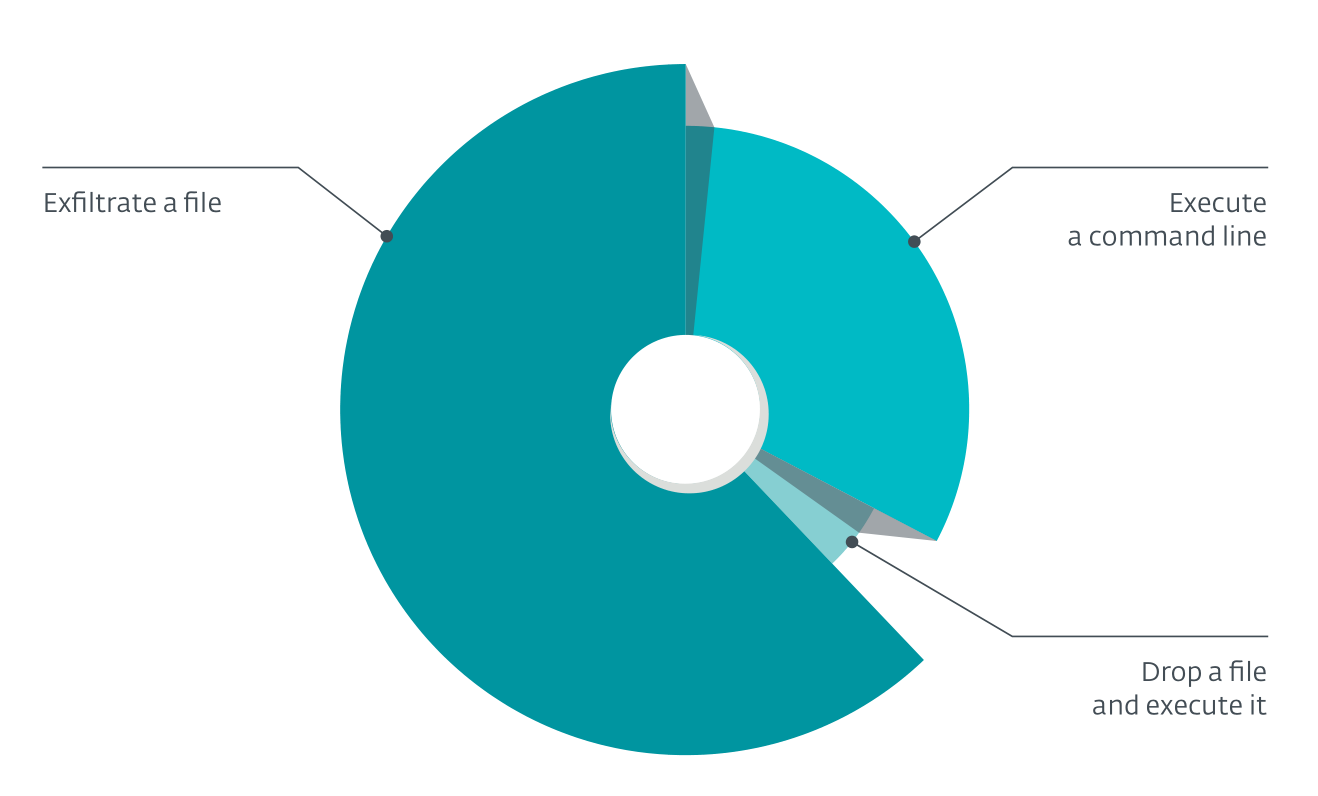
\includegraphics[height=3.5cm,width=4.6cm]{figures/commands_distrib.PNG}}
    \end{figure}
\end{frame}

\begin{frame}[fragile]{Victimology}
  According to ESET, LightNeuron development started before 2014; even if the development occurred
several years ago, LightNeuron is still used in recent compromises. These targets are in line with traditional Turla targets:
\begin{figure}
  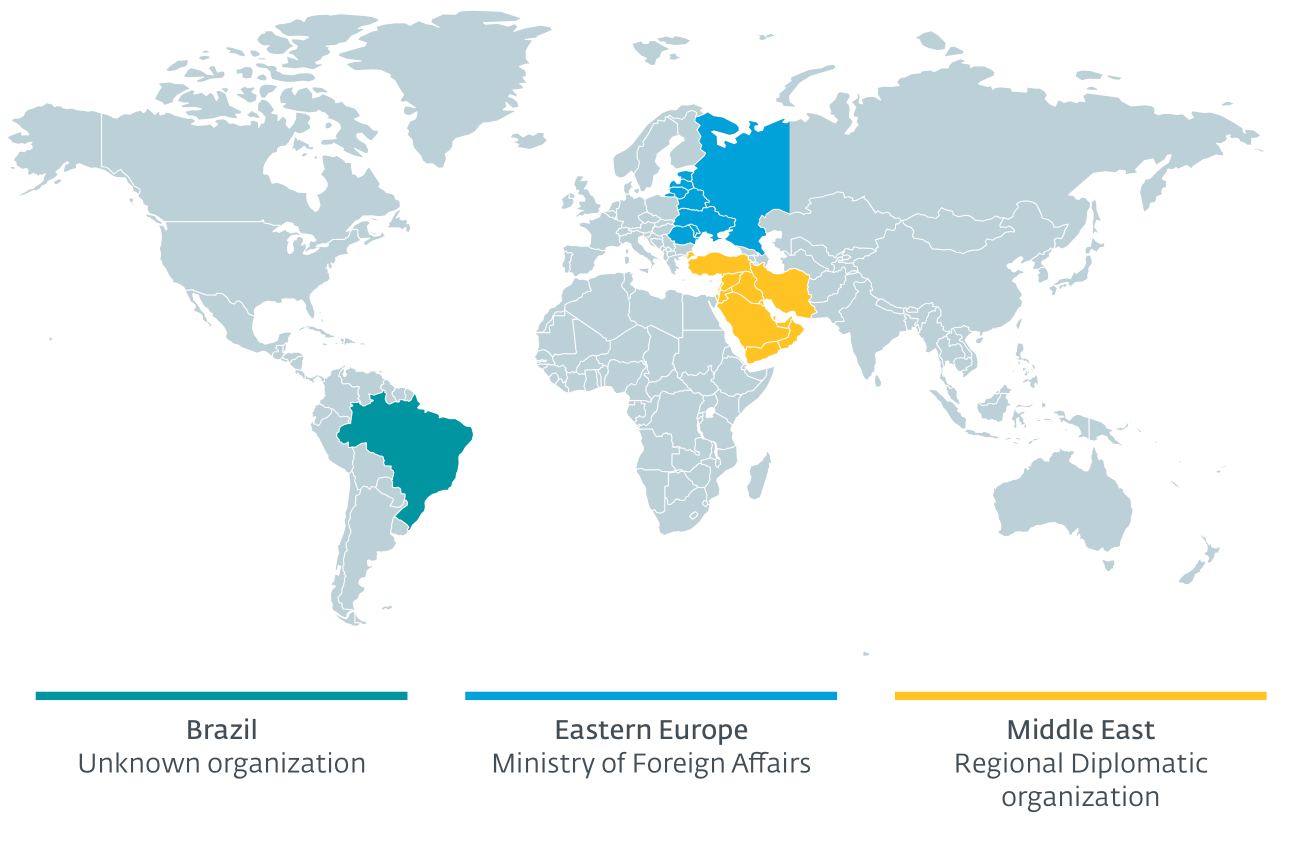
\includegraphics[width=8cm]{figures/map.PNG}
  \caption{Map of known LightNeuron victims}
\end{figure}
\end{frame}
%============================
%   3. Tools & Tactics
%============================
\section{Tools \& Tactics}

\begin{frame}
    \frametitle{Tools \& Tactics}
    \begin{enumerate}
        \item the malware
        \item the backdoor
    \end{enumerate}
\end{frame}

\begin{frame}
    \frametitle{The Malware}
    Light neuron is a rootkit
\end{frame}
%============================
%   4. Impact
%============================
%\section{Impact}

\begin{frame}
\frametitle{Impact}
    very high
\end{frame}
%============================
%   5. Countermeasures
%============================
\section{Countermeasures}

\begin{frame}[fragile]{Countermeasures i}
    \begin{itemize}
        \item The cleaning of LightNeuron is not an easy task. \textbf{Simply removing the two malicious files will break
Microsoft Exchange}, preventing everybody in the organization from sending and receiving emails.
        \item Before actually removing the files, the malicious Transport Agent should be disabled
        \item open \texttt{<ExchangeInstallFolder>/TransportRoles/Agents/agents.config} and check every DLL signature.
        \item disable the malicious Transport Agents, and after that it is possible to safely remove the infected files.
    \end{itemize}
\end{frame}

\begin{frame}[fragile]{Countermeasures ii}
Given that attackers have gained administrative privileges on the Exchange server, there are no bulletproof
        mitigations against this threat; however there are some recommendations worth to mention:
    \begin{itemize}
        \item Use dedicated accounts for the administration of Exchange servers with strong, unique passwords
        and, if possible, 2FA.
        \item Monitor closely the usage of these accounts (DLL uses a lot of log files)
        \item Restrict PowerShell execution
        \item Regulary check all the installed Transport Agents
    \end{itemize}
\end{frame}

\begin{frame}[fragile]{Microsoft’s View}
    \emph{``an attacker would need to have administrative access on an Exchange server as a member of the Exchange
     Administrator group in an organization’s Active Directory.  Exchange Administrator accounts are tightly controlled,
      and membership cannot be obtained by persuading a victim to click through a security warning or elevation request.''} \cite{Petri}
\end{frame}

%============================
%   6. Conclusions
%============================
\section{Conclusions}

\begin{frame}[fragile]{Conclusions}
    \begin{itemize}
        \item LightNeuron is another example that Turla operators
        have a large set of sophisticated, custom malware at their disposal
        \item This is the first time a malicious actor has leveraged a Microsoft Exchange Transport
        Agent to enable persistence on a mail server
        \item This technique is very interesting as it allows them to receive
        commands and exfiltrate data without any filtering.
        \item Probably not many servers have been infected in this manner, but it’s certainly wise to review Exchange server configurations to look for any unexplained transport agent.
    \end{itemize}
\end{frame}


%============================
%   Biblio
%============================

\begin{frame}[allowframebreaks]{References}

  \bibliography{biblio}
  
  %\bibliographystyle{abbrv}

\end{frame}

\end{document}
